\makeatletter
\cxset{style13}
\cxset{style87a/.style={
 chapter opening=any,
 name=Chapter,
 % positioning and float - inline is 0
 %  float right is 2
 number display=block,
 number float=right,
 number shape=starburst,
 chapter numbering=arabic,
 number spaceout=none,
 number font-size=huge,
 number font-weight=mdseries,
 number font-family=sffamily,
 number font-shape=upshape,
 number before=,
 number display=inline,
 number float=none,
% 
 number border-top-width=0pt,
 number border-right-width=0pt,
 number border-bottom-width=0pt,
 number border-left-width=0pt,
 number border-width=0pt,
%  
 number padding-left=0em,
 number padding-right=0.5em,
 number padding-top=0em,
 number padding-bottom=0pt,
  %number margin-top=, to do
 %number margin-left=0pt,  to create
 %
 number after=,
 number dot=,
 number position=rightname,
 number color=white,
 number background-color=white,
 %chapter name
 chapter display=block,
 chapter float=left,
 chapter shape=ellipse,
 chapter color=white,
 chapter background-color=sweet,
 chapter font-size= Huge,
 chapter font-weight=mdseries,
 chapter font-family=sffamily,
% chapter font-shape=upshape,
 chapter before=,
 chapter spaceout=none,
 chapter after=,
 chapter margin left=0cm,
 chapter margin top=0pt,
 %
 chapter border-width=0pt,
 chapter border-top-width=0pt,
 chapter border-right-width=0pt,
 chapter border-bottom-width=0pt,
 chapter border-left-width=0pt,
% 
 chapter padding-left=0pt,
 chapter padding-right=0pt,
 chapter padding-top=0pt,
 chapter padding-bottom=0pt,
  %chapter title
 title font-family=sffamily,
 title font-color=black!80,
 title font-weight=bfseries,
 title font-size=huge,
 chapter title align=none,
 title margin-left=1cm,
 title margin bottom=1.3cm,
 title margin top=25pt,
 % title borders
 title border-width=0pt,
 title padding=0pt,
 title border-color=black!80,
% title border-top-color=spot!50,
% title border-top-width=20pt,
 title border-left-color=black!80,
 title border-left-width=2pt,
 title border-color=black!80,
 title padding-top=10pt,
 title padding-bottom=10pt,
 title padding-left=10pt,
 title padding-right=0pt,
% title border-right-color=spot!50,
% title border-right-width=20pt,
% title border-bottom-color=spot!50,
% title border-bottom-width=20pt,
 %
 chapter title align=left,
 chapter title text-align=left,
 chapter title width=0.8\textwidth,
 title before=,
 title after=,
 title display=block,
 title beforeskip=,
 title afterskip=,
 author block=false,
 section font-family=rmfamily,
 section font-size=LARGE,
 section font-weight=bfseries,
 section indent=0pt,
 epigraph width=\dimexpr(\textwidth-2cm)\relax,
 epigraph align=center,
 epigraph text align=center,
 section color=spot!50,
 section font-weight=bfseries,
 section align=left,
 section number after=\hskip10pt,
 section font-family=sffamily,
 section numbering prefix=\@arabic\c@chapter.,
 epigraph rule width=0pt,
 header style=plain}}
 \makeatother
 
\cxset{style87a}


\def\authorblockformat{\raggedright}
\cxset{author block=false,
          author names=Dr Y. Lazarides}
\MakePercentComment

\chapter[Simulation of transient flows in pipes with different material characteristics]{\color{spot!50}Simulation of transient flows in pipes with different material characteristics}
\thispagestyle{plain}
\pagestyle{headings}

This short document provides background information to the study of transient flows in plumbing systems and then
summarizes the results of a simulation carried out for typical hotel guest room water supply systems in order
to provide a recommendation as to the incorporation or not of water hammer arrestors.


\section{Introduction}

Hydraulic transients in piping systems occur when steady-state conditions at a given point in the pipeline start changing with time. This would normally occur when a valve is closed quickly or a pump is switched-off abruptly (mains power failure).  When a valve is suddenly closed the water column continues to move until the end of the pipe, when it will hit the wall and reflect back. In a large diameter pipe such as a 1000 mm pipe transporting water from a water reservoir to a city the sudden pump stop, maybe due to a mains failure and can create considerable forces. In the case of a plumbing system solenoid valves at washing machines might cause similar issues. 

\section{The Joukowsky equation}

The problem was first scientifically studied by Joukowsky and the background theory can be found in standard fluid dynamics handbooks.

The pressure change \(\Delta p_{Jou}\) in a fluid caused by an instantaneous
change in flow velocity $\Delta v$ is calculated
by:

\begin{equation}
\Delta p_{Jou} = \rho a \Delta v
\label{jou}
\end{equation}

where,

The $\Delta p_{Jou}$ formula is referred to
as the Joukowsky equation. As
well as $\Delta v$, equation (\ref{jou}) contains
the density $\rho$ and wave
propagation velocity $a$. The relationship
only applies to the period
of time in which the velocity
change $\Delta v$ is taking place. If
$\Delta v$ runs in opposite direction to
the flow, the pressure will rise,
otherwise it will fall. 

The parameter $a$ is a factor both of the pipe Modulus of Elasticity, as well as the fluid being transported and is the main factor in producing different outcomes for different pipe materials.

\section{Plastic Piping Water Hammer Resistance}

The ability of a plumbing pipe to dissipate energy due to surge in water pressure is based on the pipe’s modulus of elasticity, a measure of material stiffness. A higher modulus of elasticity means the material is more rigid. Copper pipe is 180 times more rigid than PEX pipe.

The surge pressure that causes water hammer can produce instantaneous pressures of 300 to 400 psig, which can, over time, cause damage to \textit{rigid} pipes, such as copper tubing, fittings, fixtures, and hot water tanks. 

In summary, the flexibility of PEX pipe allows the pipe itself to absorb energy from pressure surges and eliminate or reduce  the occurence of water hammer. It is notable that a number of US States codes, now qualify the requirement for the use of water-hammer arrestors so that they exclude plastic piping. We quote for example the North Carolina 2012 NC Plumbing Code, below:

\cxset{quotation font-size=\large, quotation above=10pt, quotation left margin=\parindent}
\begin{quotation}
\textbf{604.9 Water hammer}. The flow velocity of the water distribution system shall be controlled to reduce the possibility of water hammer. A water-hammer arrestor shall be installed where quick-closing valves (example: clothes washers, dish-washers, ice makers) and metallic piping is used. The water hammer arrestor shall not be required on any valves where plastic pipe is used for water distribution piping. Water-hammer arrestors shall be installed in accordance with the manufacturer’s specifications. Water-hammer arrstors shall conform to |ASSE 1010|.\footnote{\protect\url{http://www.ncdoi.com/OSFM/Engineering_and_Codes/Documents/2012_NCBuildingCode_amendments/PlumbingCode-2012NCAmendments100517.pdf}} 
\end{quotation}

It is also instructive to note that no current or past European standard specified the use of water hammer arrestors, but left the decision to the designer, who was expected to have resolved the issue of surge pressures via a judicious selection of water flow velocities, correct spacing of supports and by fitting slow acting solenoid valves where necessary. 

\section{Computer simulations}

Most computer programs are based on the so-called method of characteristics. This
method is an elegant and efficient way of solving the basic equations for unsteady flow
in pipelines. The method takes advantage of the fact that all variations in pressure and
flow move with the same velocity as the wave c and that all these variations in principle
are connected according to the Joukowsky equation, which in this context is extended to
incorporate friction.

\subsection{Model Definition}

The piping system in the steady state consists of a reservoir/riser with branch manifold
and |PEX| pipe from the manifold to the plumbing fixture or copper |PPR| pipe from riser
to to the plumbing fixture.

The valve in this model closed instantaneously. As a result of the compressibility of the
water and the elastic behavior of the pipe a sharp pressure pulse is generated travelling
upstream of the valve.

\subsection{Computer Simulation setup}

The simulation software were set up, so that at a distance $z_{0} = 1.5$ m from the riser there is a virtual pressure sensor or pressure measurement point, that  samples measurements at 0.01 second intervals 
(100 Hz ) for a duration of 1.5 second from the valve closing . 

The piping riser acts as a constant pressure source with a set pressure of $p_0 = 4$ bar. As an initial condition the valve is open and
water is flows steadily at a low rate of $Q_0 = 0.5$ \si{\liter\per\second}.  At time $t = 0$ s the valve is
closed instantaneously initiating the pressure surge. The simulation was preformed on
|PEX|, |PPR| and |copper| for 2 and 7 meter lengths between the riser and the valve and the
pressure measured at 400 points along the pipe length. The results are presented graphically at the next section.


\subsection{Results}

The excess pressure history, $\Delta p=p-p_0$, as measured at the pressure sensor located at $z_0$
is depicted in Figure\ref{pex1}\&\ref{pex2} for |PEX pipe|. Figure~\ref{ppr1}\&\ref{ppr2} for PPR pipe and Figure \ref{co1}\&\ref{co2} for the copper pipe simulation.

The excess pressure waves along the pipe at time t = 0 to 1.5 s with 0.01s interval is
depicted in Figure\ref{pex3}\&\ref{pex4} for PEX pipe , Figure \ref{ppr3}\&\ref{ppr4} for PPR pipe and Figure \ref{co3}\&\ref{co4} for copper pipe.


\begin{figure}[htbp]
\hspace*{-0.1\textwidth}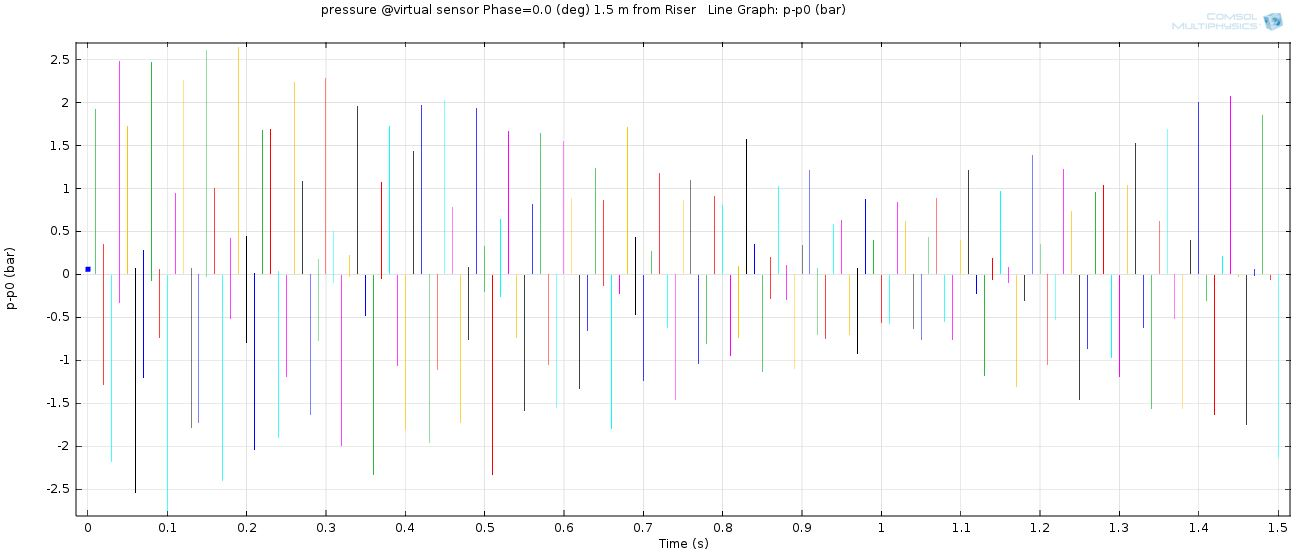
\includegraphics[width=1.2\textwidth]{./water-hammer/PEX/PEX-2-sensor}
\caption{Excess pressure history for \texttt{PEX} pipes for length 2 m (sensor).}
\label{pex1}
\end{figure}

\begin{figure}[htbp]
\hspace*{-0.1\textwidth}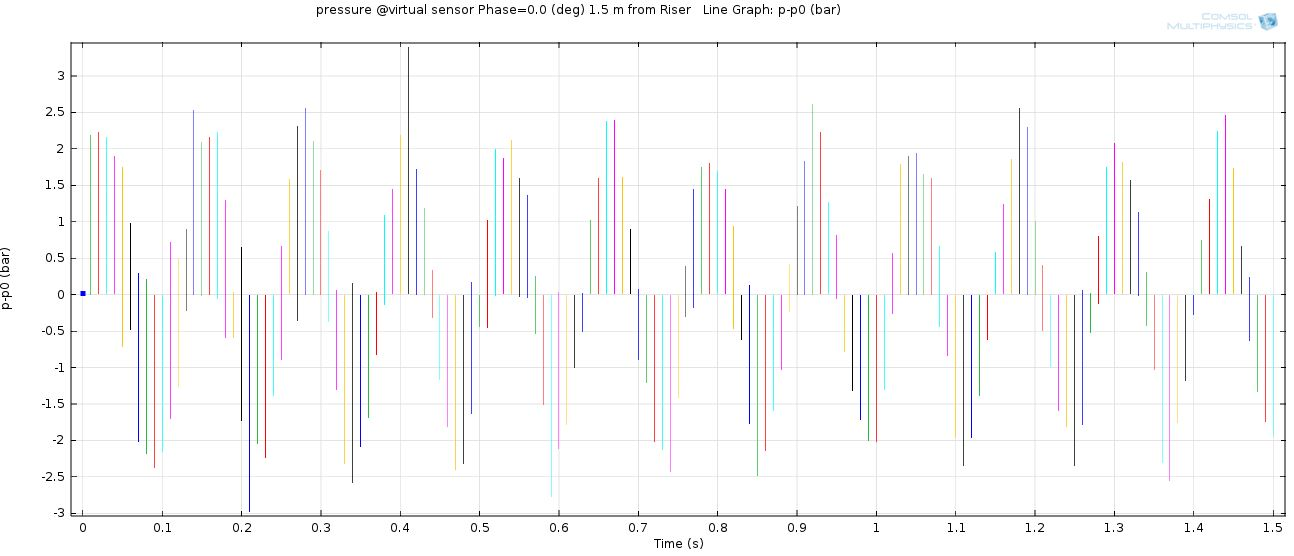
\includegraphics[width=1.2\textwidth]{./water-hammer/PEX/PEX-7-sensor}
\caption{Excess pressure history for \texttt{PEX} pipes for length 7 m (sensor).}
\label{pex2}
\end{figure}

\begin{figure}[htbp]
\hspace*{-0.1\textwidth}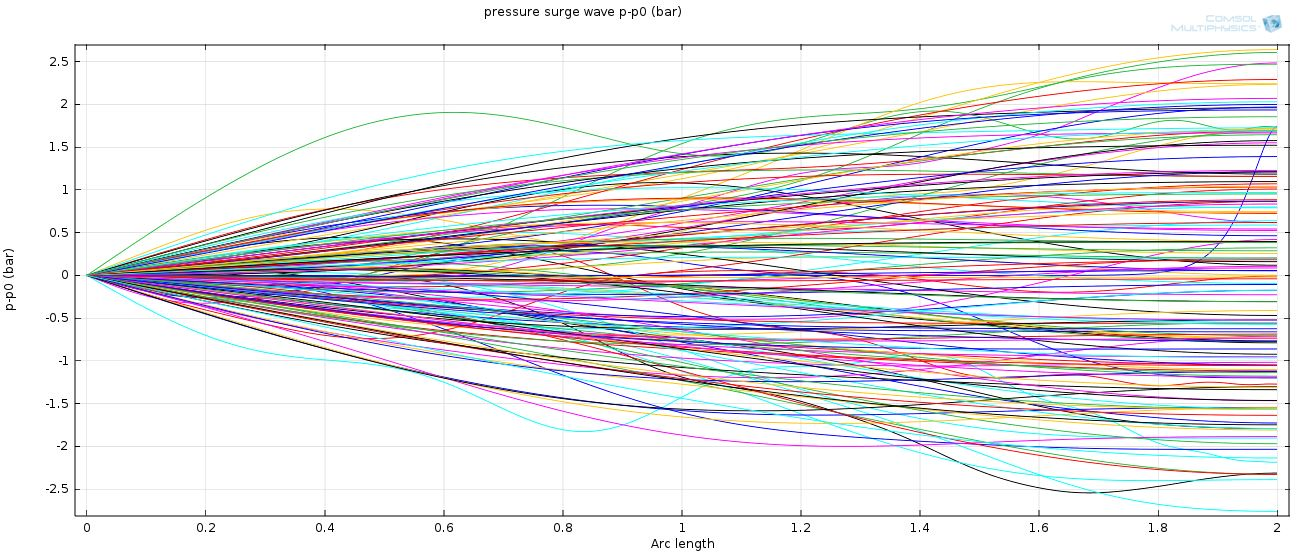
\includegraphics[width=1.2\textwidth]{./water-hammer/PEX/PEX-2}
\caption{Excess pressure history for \texttt{PEX} pipes for length 2 m.}
\label{pex3}
\end{figure}

\begin{figure}[htbp]
\hspace*{-0.1\textwidth}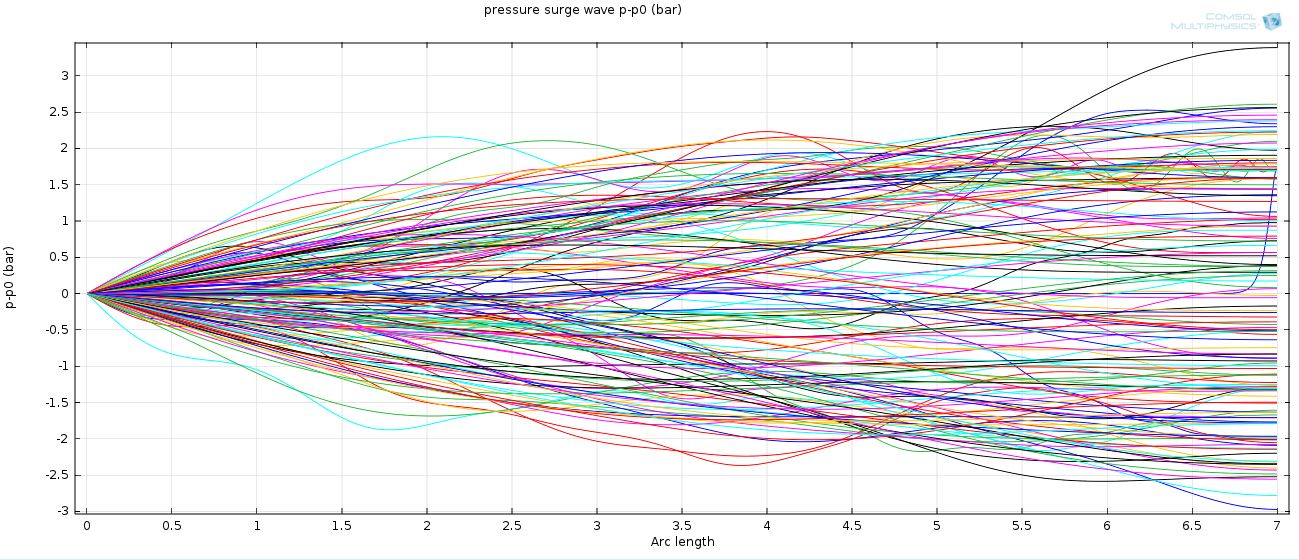
\includegraphics[width=1.2\textwidth]{./water-hammer/PEX/PEX-7}
\caption{Excess pressure history for \texttt{PEX} pipes for length 7 m.}
\label{pex4}
\end{figure}


\begin{figure}[htbp]
\hspace*{-0.1\textwidth}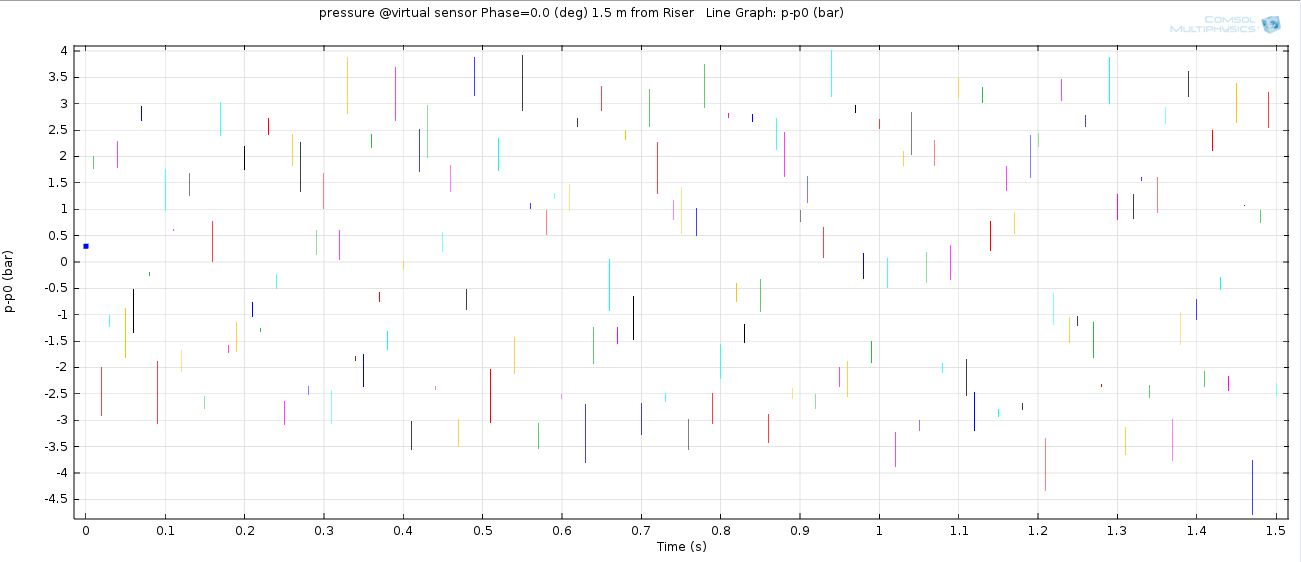
\includegraphics[width=1.2\textwidth]{./water-hammer/PPR/PPR-2-sensor}
\caption{Excess pressure history for \texttt{PPR} pipes for length 2 m (sensor).}
\label{ppr1}
\end{figure}

\begin{figure}[htbp]
\hspace*{-0.1\textwidth}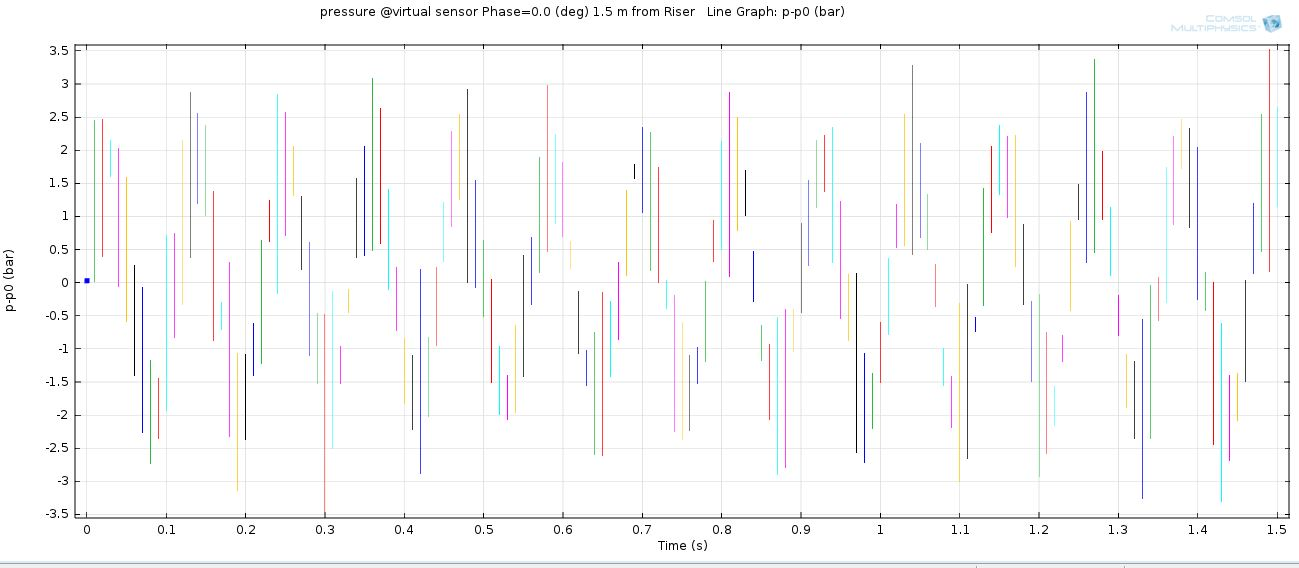
\includegraphics[width=1.2\textwidth]{./water-hammer/PPR/PPR-7-sensor}
\caption{Excess pressure history for \texttt{PPR} pipes for length 7 m (sensor).}
\label{ppr2}
\end{figure}

\begin{figure}[htbp]
\hspace*{-0.1\textwidth}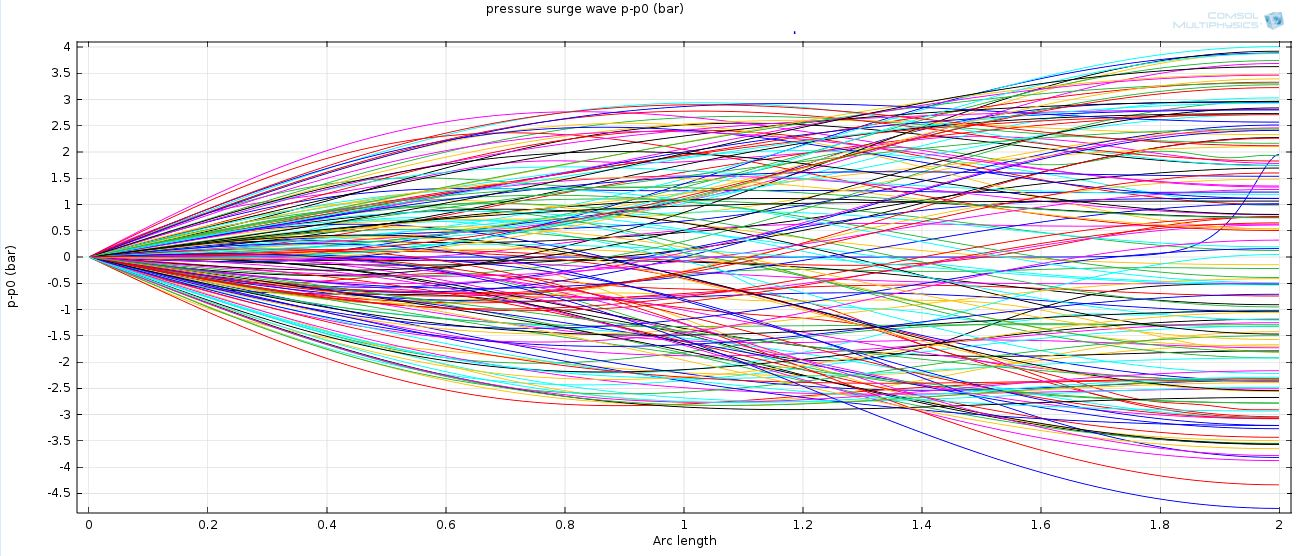
\includegraphics[width=1.2\textwidth]{./water-hammer/PPR/PPR-2}
\caption{Excess pressure history for \texttt{PPR} pipes for length 2 m.}
\label{ppr3}
\end{figure}

\begin{figure}[htbp]
\hspace*{-0.1\textwidth}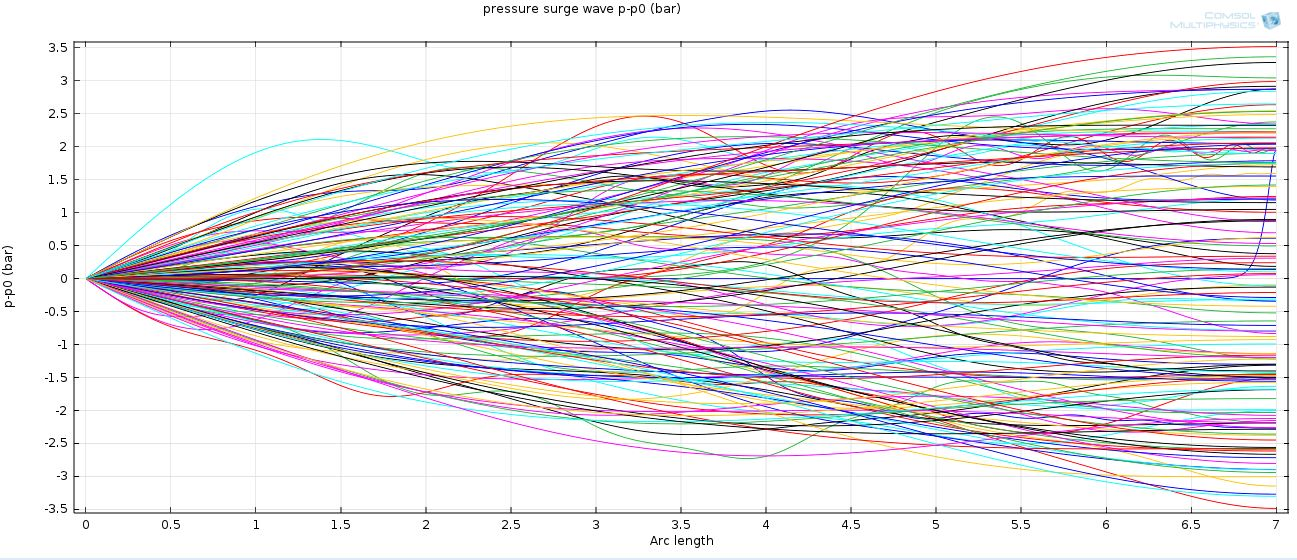
\includegraphics[width=1.2\textwidth]{./water-hammer/PPR/PPR-7}
\caption{Excess pressure history for \texttt{PPR} pipes for length 7 m.}
\label{ppr4}
\end{figure}

\begin{figure}[htbp]
\hspace*{-0.1\textwidth}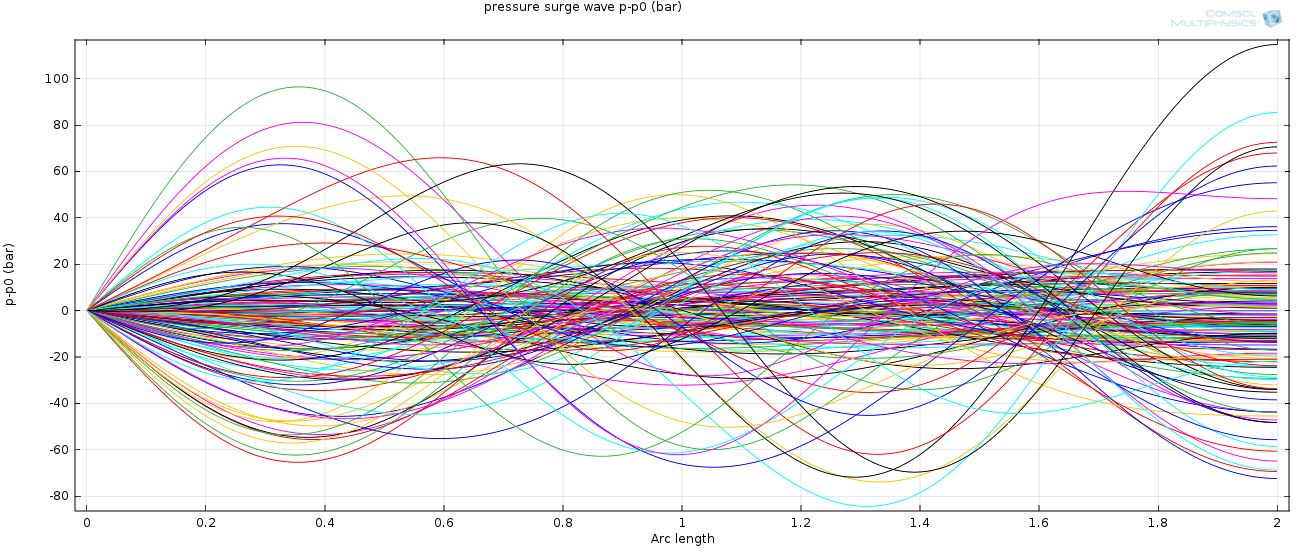
\includegraphics[width=1.2\textwidth]{./water-hammer/copper/CO-2}
\caption{Excess pressure history for \texttt{copper} pipes for length 2 m.}
\label{co1}
\end{figure}

\begin{figure}[htbp]
\hspace*{-0.1\textwidth}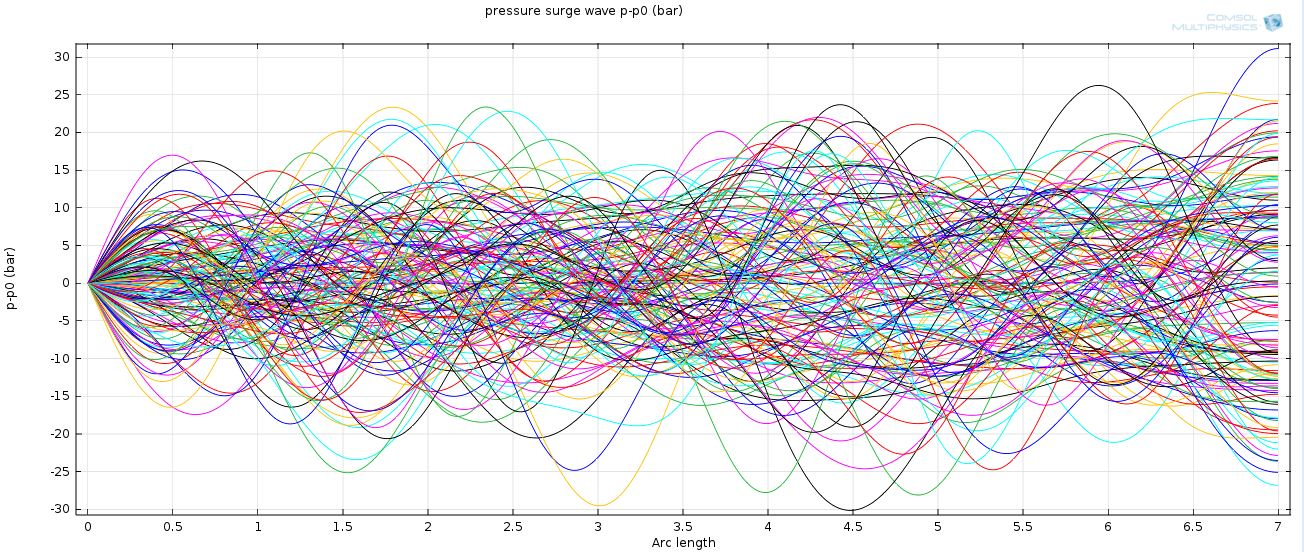
\includegraphics[width=1.2\textwidth]{./water-hammer/copper/CO-7}
\caption{Excess pressure history for \texttt{copper} pipes for length 7 m.}
\label{co2}
\end{figure}

\begin{figure}[htbp]
\hspace*{-0.1\textwidth}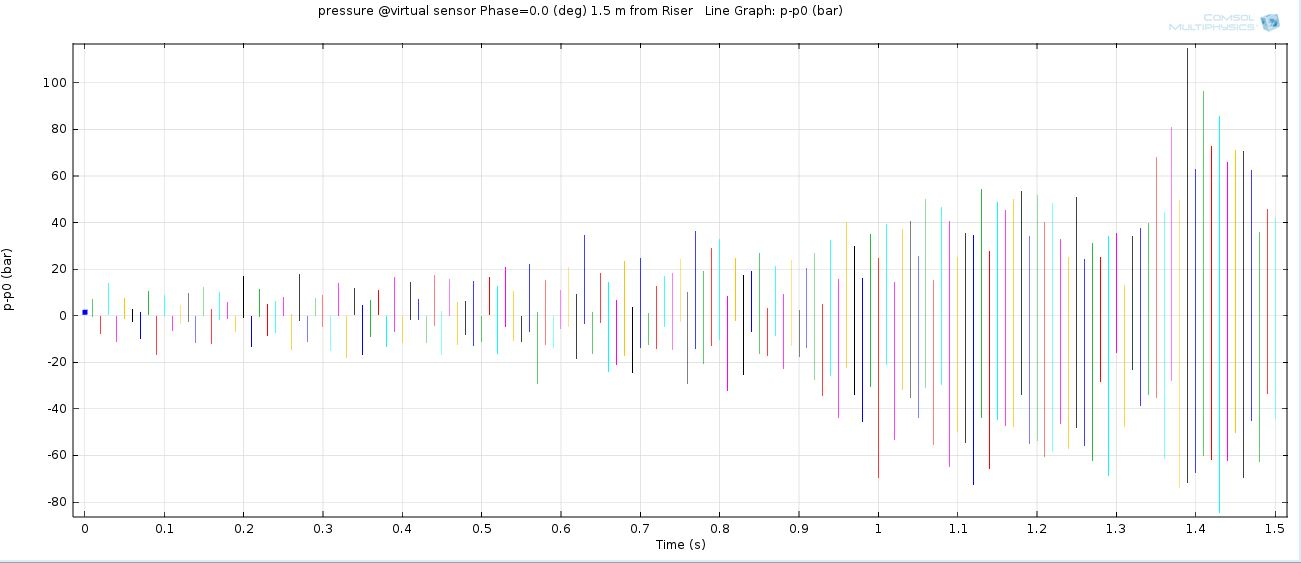
\includegraphics[width=1.2\textwidth]{./water-hammer/copper/CO-2-sensor}
\caption{Excess pressure history for \texttt{copper} pipes for length 2 m (sensor).}
\label{co3}
\end{figure}

\begin{figure}[htbp]
\hspace*{-0.1\textwidth}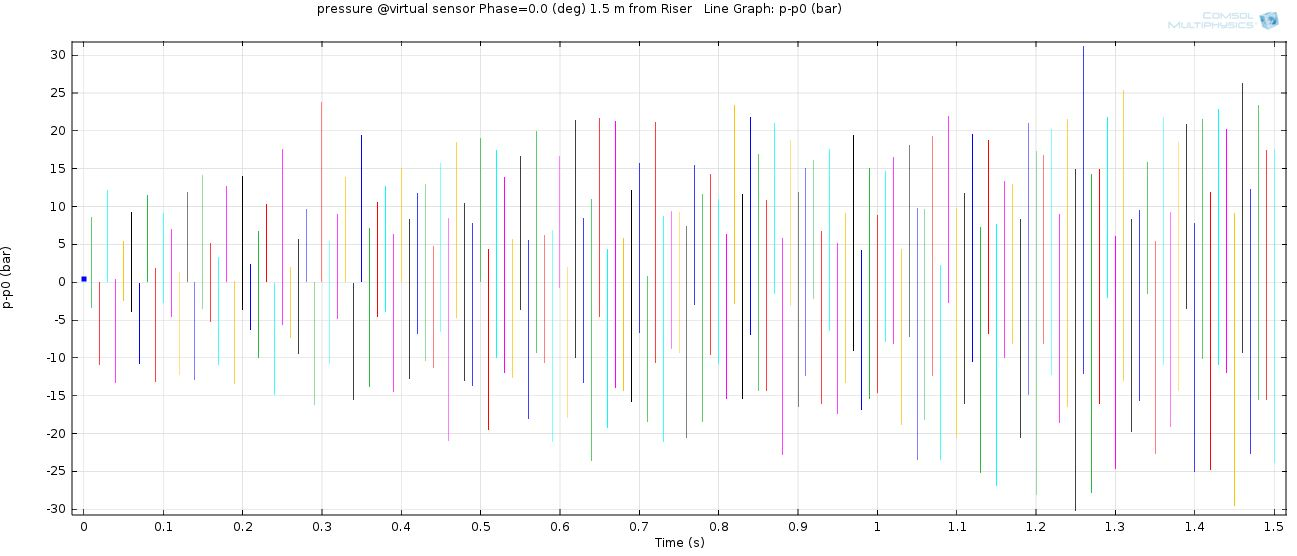
\includegraphics[width=1.2\textwidth]{./water-hammer/copper/CO-7-sensor}
\caption{Excess pressure history for \texttt{copper} pipes for length 7 m (sensor).}
\label{co4}
\end{figure}




\chapter[Conclusions and Recommendations as to the necessity of installing water-hammer arrestors in a plumbing system utilizing \texttt{PEX} piping]{\color{spot!50} Conclusions and Recommendations as to the necessity of installing water-hammer arrestors\\ in a plumbing system\\ utilizing \texttt{PEX} piping}

It can be observed both from the first order calculations using the Joukowski equation, as well as the computer simulation, that where |PEX| piping is employed, the flexibility of the material absorbs a substantial portion of the pressure-surge resulting in overpressures that are considerably lower than those obtained with copper. These pressures are within the acceptable range for the installation.

The calculations as presented are conservative in that they have assumed that a valve closes instantaneously in zero seconds. In reality in hotel guest rooms there are no fast closing valves such as the solenoids used for example to serve washing machines in apartments and valves will be manually closed within a time frame of seconds which will result in substantially lower surge pressures.

In addition to the results of the study commercial accumulators require a substantial force to raise the piston of the accumulator. 
It is likely that  the pex pipe a will absorb most of the pressure wave and not the accumulator, even if employed. 

 Our recommendation is to minimize the costs to the Project and not provide the water hammer arrestors. We note that the HLS DSE-JV has a financial interest to \textit{install} the water hammer arrestors, rather than omit them,  as they were originally excluded from our Contract. The recommendation to omit them has been carried out in good faith, and at no cost to the Client as a Value Engineering proposal estimated to save costs in the region of AED~1,000,000.00.




